\section{Sharpening in the spatial domain}

\subsection{Section1}
\begin{figure}[ht]
\centering
	\subfigure[Base Cameraman image]{
	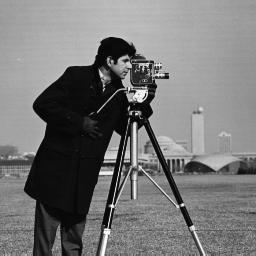
\includegraphics[width=0.45\linewidth]{question4/1_camBase}
	}
	\subfigure[Original image - Blurred image]{
	
\includegraphics[width=0.45\linewidth]{question4/1_cam_highBoost}
	}
\end{figure}

\subsection{Section2}
\begin{figure}[ht]
\centering
	\subfigure[High-boosted image, A=1.0]{
	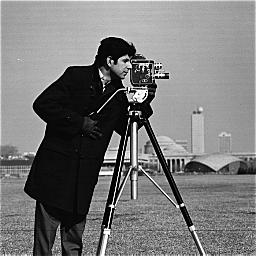
\includegraphics[width=0.45\linewidth]{question4/2_cam_highBoost_10}
	}
\end{figure}


\subsection{Section3}
\begin{figure}[ht]
\centering
	\subfigure[High-boosted image, A=0.5]{
	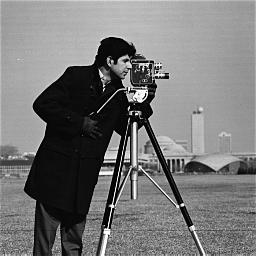
\includegraphics[width=0.45\linewidth]{question4/3_cam_highBoost_05}
	}
\end{figure}

\begin{figure}[ht]
\centering
	\subfigure[High-boosted image, A=1.5]{
	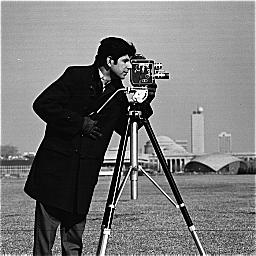
\includegraphics[width=0.45\linewidth]{question4/3_cam_highBoost_15}
	}
	\subfigure[High-boosted image, A=4.0]{
	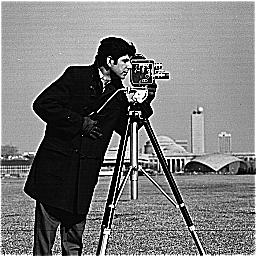
\includegraphics[width=0.45\linewidth]{question4/3_cam_highBoost_40}
	}
\end{figure}

\subsection{Discussion questions}

\subsubsection{What does the subtracted image look like? What frequency components from the original image are
preserved in the subtracted image? Why?}
The subtracted image looks like an outline of the original image (i.e. edges are preserved). This is because high frequency components are preserved in the subtraction image. This occurs because the Gaussian filtered image eliminates high frequency components, and thus high frequency is all that is left when it is subtracted from the original image.

\subsubsection{What does the resulting image look like? How does it differ from the original image? Explain why it
appears this way}
The high boosted image has sharper edges than the original. This is because the prominence of the high frequency components is being increased by adding another set of them (i.e. the subtracted image).

\subsubsection{Compare the results produced by adding the subtracted image to the original image and that produced
by adding half of the subtracted image to the original image. How does it differ? Explain why it
appears this way}
The edges are less prominent in the image with half the subtracted image added. This is because the high frequency components are accentuated less. However, high frequency noise is also less prominant than the half image.

\subsubsection{What does multiplying the subtracted image by a factor less than one accomplish? What about greater
than one}

By multiplying it by a factor less than one, edges are not as sharp, but high frequency noise is also less magnified. With a value greater than one, the reverse it true.
